%!TEX root = /Users/nebolsin/Documents/MSU/Graduate Work/tex/main.tex
\section{Обзор существующих программных сред, использующихся в прикладных научных исследованиях} 
\label{review}

В данном разделе кратко описываются пять PSE, которые используются учеными при решении задач в конкретных узких областях. Эти примеры подчеркивают разнообразие междисциплинарных сообществ, что позволяет выделить и проанализировать основные требования к РВС.

\subsection{WBCSim (исследование композитов из древесины)}

WBCSim --- это широко доступная и простая в использовании прототипная PSE, которая предназначена для увеличения продуктивности ученых проводящих исследования композитных материалов, основанных на древесине, путем предоставления программ на языке FORTRAN, решающих различные научные проблемы в области разработки композитных материалов. WBCSim в настоящее время предоставляет доступ через интернет для запуска из командной строки имитаций, разработанных в рамках программы Wook-Based Composites (WBC) в Virginia Tech. WBCSim использует всемирную доступность веб-а чтобы организовать работу с кодом имитаций для ученых и инженеров, не работающих в лабораториях Virginia Tech. Система конвертирует выходные данные вычислений в язык моделирования виртуальной реальности (VRML) для визуализации результатов имитаций. WBCSim имеет две цели: (1) увеличение продуктивности исследовательской группы WBC путем улучшения программной среды; (2) функционирование в качестве прототипа для разработки и реализации PSE большего масштаба. Коды имитаций, использующихся в качестве тестов, написаны на языке FORTRAN~77 и практически не требют взаимодействия с пользователем. Вся передача данных организована при помощи файлов специального формата, что делает трудным использование кода. WBCSim скрывает все это в реализации сервера и позволяет пользователям предоставить входные данные, запустить имитацию удаленно и просмотреть результаты как в текстовом, так и в графическом формате.

WBCSim содержит четыре модели имитаций, интересных для ученых, изучающих производство композитных материалов из древесины --- имитацию роторной сушилки (RDS), радио-частотное прессование (RFP), анализ композитных материалов (CMA) и формирование сплетений из частиц (MAT). Имитация роторной сушилки была разработана для поддержки разработок сушильных систем для дресесных частиц, используемых в производстве древесно-стружечных и древесно-волокнистых плит. Роторные сушилки используются примерно в 90\% таких процессов. Модель радио-частотного прессования была разработана для имитации соединения древесного шпона в многослойный композит, где энергия, необходимая для вулканизации клея генерируется электрическим полем высокой частоты. Анализ композитных материалов используется для определения прочности многослойных материалов, таких как фанера. Моделирование формирования сплетений имитирует процесс спутывания древесных волокон при спрессовывании и используется для определения свойств древесных композитов. Эта модель необходима для всех прочих моделей производственного процесса, так как они требуют параметры материала в качестве входных данных.

\begin{figure}
  \centering
  	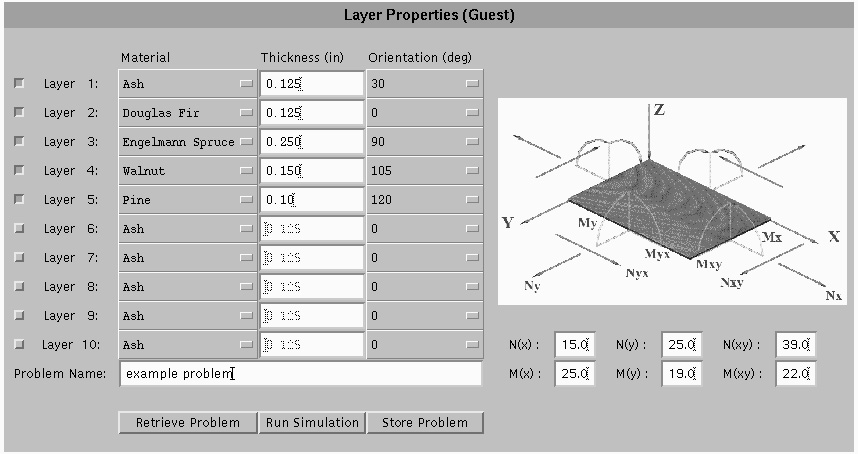
\includegraphics[width=14cm]{images/wbcsim-screenshot.png}
	\caption{Интерфейс CMA-анализа в WBCSim PSE}
	\label{fig:wbcsim-screenshot}
\end{figure} 

Программная архитектура WBCSim имеет три слоя: (1) существующий имитационный код и различные средства визуализации и оптимизации, возможно, запущеные удаленно; (2) пользовательский интерфейс; (3) связующий слой, который распределяет запросы пользователей к имитациям и другим средствам и возвращает результат. Эти три слоя называются <<слой разработчика>>, <<слой пользователя>> и <<слой сервера>> соответственно. Слой разработчика состоит в основном из существующего имитационного кода, на котором основан WBCSim. Серверный слой ожидает от программы из слоя разработчика использования определенных форматов входных и выходных данных. То есть, имитационные программ <<обернуты>> в специальные Perl-скрипты и для каждой новой программы необходимо писать свою, новую <<обертку>>. Клиентский слой состоит из Java-апплетов и отвечает за пользовательский интерфейс и взаимодействие с серверным слоем. Обычно только этот слой выполняется на пользовательском компьютере. Серверный слой --- это ядро WBCSim, он отвечает за запуск имитаций и за взаимодействие с пользовательским интерфейсом. Приложения WBCSim требуют сложного управления вычислениями: серверный слой, написанный на языке Java, одновременно следит за несколькими имитациями и принимает запросы от многих пользователей, а также получает и обрабатывает сообщения, которые показывают прохождение важных точек в вычислениях (например, получение промежуточного значения). Графические результаты имитаций передаются пользователю при помощи HTTP-сервера.

\textbf{Выводы:} распрделенная вычислительная среда должна поддерживать работу с уже существующим программным кодом, который невозможно переписать под нужны системы. Для этого предлагается предусмотреть систему «оберток», использующую интерпретируемый язык программирования и адаптирующую интерфейс существующих программных модулей под требования, необходимые для использования их в вычислительной среде. Кроме того, среда должна поддерживать одновременное проведение нескольких вычислений и иметь механизмы для получения промежуточных результатов вычислений.

\subsection{VizCraft (авиационное моделирование)}
\begin{figure}
  \centering
    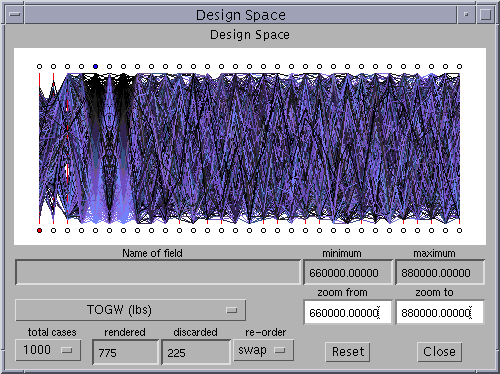
\includegraphics[width=12cm]{images/vizcraft-screenshot.png}
  \caption{Визуализация 156 моделируемых параметров в 29 измерениях в окне просмотра дизайна VizCraft}
  \label{fig:vizcraft-screenshot}
\end{figure}       

VizCraft --- это PSE для поддержки авиационных дизайнеров на стадии концептуального дизайна. На этой стадии дизайн самолета представляется вектором, содержащим от 10 до 30 параметров. Цель данного этапа заключается в нахождении такого вектора, который минимизирует некую целевую функцию и в то же время удовлетворяет ряду ограничений. В VizCraft интегрирован код для рассчетов и средства визуализации, позволяющие как оценить единичный вариант дизайна, так и сравнить его с другими вариантами. VizCraft позволяет легко переключаться между режимом просмотра набора параметров и режимом визуализации формы самолета, соответсвующей данным параметрам. В случае нарушения ограничений, пользователь может легко увидеть, какие именно ограничения нарушаются. VizCraft --- это дизайнерский инструмент, применяемый на этапе концептуального дизайна, целью которого является предоставление среды, в которой объединены вычисления и визуализация. Дизайнеру предоставляется возможность размышлять в терминах решения проблемы, а не просто использовать визуализацию чтобы просмотреть результаты вычислений.

VisCraft предоставляет графический интерфейс к модельному коду высокоскоростного гражданского транспорта (HSCT), который использует 29 переменных и 68 реальных ограничений. Это огромный код на C и FORTRAN, который вычисляет геометрическую форму самолета в 3D, общий подъемный вес самолета и многи другие вещи. VizCraft отображает платформу HSCT (общий вид), аэродинамические поверхности, углы атаки крыльев и цветовую информацию о нарушении ограничений. Для облегчения работы с ограничениями они сгруппированы в аэродинамические ограничения, геометрические ограничения и ограничения производительности. Параметры дизайна и соответсвующий подъемный вес, а также нарушения ограничений, отображаются с использованием активных параллельных координат. Несмотря на то, что интеграция междисциплинарного кода HSCT в PSE достаточно сложна, сила и уникальность среды VizCraft заключается в поддержке визуализации данных высокой размерности (см. рис.~\ref{fig:vizcraft-screenshot}).

\textbf{Выводы:} распределенная вычислительная среда должна иметь возможность подключения средств визуализации и сравнения результатов различных вычислений.  

\subsection{L2W (анализ водоразделов)}
\begin{figure}
  \centering
    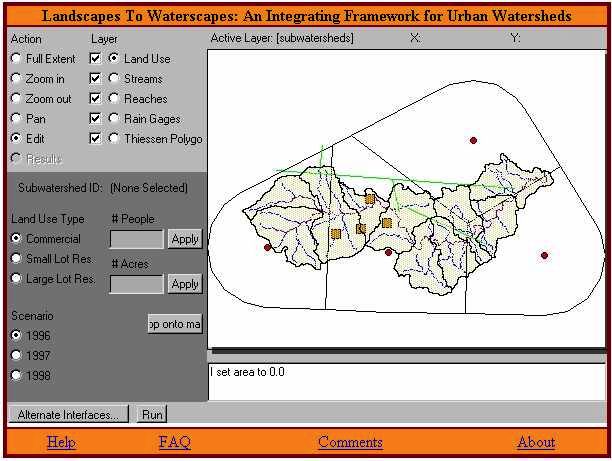
\includegraphics[width=10cm]{images/l2w-screenshot.png}
  \caption{Интерфейс принятия решений в L2W PSE, отображающий водораздел реки Upper Roanoke в Юго-Западной Вирджинии}
  \label{fig:l2w-screenshot}
\end{figure}

L2W (Landscapes to Waterscapes) --- это PSE для анализа землепользования и управления водоразделами. L2W оргаризует и унифицирует доступ к большому набору приложений, обычно использущихся при моделировании экосистем (гидрологических, экономических и биологических). Эта среда предоставляет web-интерфейс исследователям водоразделов и другим пользователям для изучения влияния землепользования на гидрологическую, экологическую и экономическую ситуацию. Управление водоразделами --- это широкая концепция, включающая в себя планы и требования по контролю за водными и другими ресурсами в данном водоразделее.

Архитектура среды L2W основана на интеграции существующего программного ообеспечения в области гидрологии, экономики и биологии в единую систему. Технологии геоинформационных систем (GIS) позволяют совместить гидрологические и экономические модели с интуитивно понятным пользовательским web-интерфейсом. Использование геоинформационных технологий в PSE позволяет создать более реалистичную систему в которой пользователь может создать сценарий изменения землепользования в какой-то местности, основываясь на реальных характеристиках. Из всех PSE, описанных в этом разделе, уникальность L2W заключается в том, что она построена на базе геоинформационных технологий. На данный момент в L2W интегрирован код гидрологического анализа поверхностей и экономические модели, позволяющие рассчитать эффект от постройки новых поселений. Специалисты в области живой природы и биологи также участвуют в проекте, но их программное обеспечение пока не полностью интегрировано в систему.

\textbf{Выводы:} поддержка геоинформационных сервисов повышает степень удобства использования вычислительной среды во многих областях науки.

\subsection{\SW (моделирование беспроводных систем связи)}
\begin{figure}
  \centering
    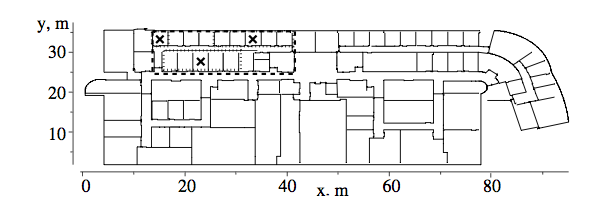
\includegraphics[width=8cm]{images/s4w-screenshot.png}
  \caption{Пример плана в \SW, показывающего наилучшее местоположения трех передатчиков для покрытия восемнадцати комнат и коридора}
  \label{fig:s4w-screenshot}
\end{figure}      

\SW --- это ориентированная на совместную работу PSE для моделирования и анализа широкополосных беcпроводных коммуникационных систем. В отличие от описанных выше систем, \SW рассчитана на работу в условиях когда высокоточные модели распространения сигналов и каналов связи разрабатываются параллельно с использованием системы; это накладывает определенные ограничения на архитектуру и реализацию среды (см. Сценарий 1 во введении). В \SW есть возможность загрузки 3D модели исследуемых помещений и применения большого количества моделей распространения радиосигналов. Например, при организации коммерческой беспроводной сети, существуют бюджетные ограничения на количество используемых ресурсов, таких как передатчики и радиоканалы. \SW позволяет инженерам автоматически запускать имитации, чтобы максимизировать покрытие или пропускную способность или минимизировать стоимость. Более того, в отличие от других существующих инструментов, \SW позволяет пользователю загрузить результаты реальных измерений мощности радиосигнала и использовать эти данные для улучшения качества имитационных моделей. При помощи этих данных система корректирует существующие модели распространения сигналов, что увеличивает точность вычислений. И, наконец, \SW имеет возможность оптимизировать размещение каждого элемента беспроводной системы в данном окружении основываясь на критерии максимального покрытия, качества сервиса или стоимости.

Несмотря на то, что существуют примитивные программные средства для моделирования сотовых систем, ни одно из них не имеет адекватной модели для эмуляции широкополосных беспроводных систем, а также их модели не учитывают эффект отраженных сигналов от зданий и других рукотворных объектов. Более того, существующие средства не позволяют использовать в них новые модели, визуализировать результаты вычислений, использовать оптимизационные циклы для моделей, проверять модели, сравнивая их с результатами реальных измерений и обрабатывать результаты, полученные в большой серии экспериментов. 

\SW разработана, чтобы увеличить производительность по трем направлениям --- программную производительность, поизводительность конечного продукта и производительность дизайнеров. Прекрасная программная производительность обеспечивается: (1) разработкой значительно улучшенных моделей беспроводных коммуникаций; (2) созданием имитационных систем, состоящих из компонентов беспроводных моделей и оптимизатора; (3) прозрачным использованием высокопроизводительных параллельных вычислений и доступом к распределенным ресурсам. Отличная производительность готового продукта (реальной беспроводной системы) обеспечивается использованием оптимизации для разработки \emph{оптимального}, а не просто \emph{подходящего} решения. Увеличение производительности дизайнеров является прямым следствием использования PSE, целью которой является облегчение труда дизайнера и автоматизация различных шагов.

\textbf{Выводы:} распределенная вычислительная среда должна поддерживать изменение и улучшение вычислительных компонентов за счет гибкой системы управления форматами входных и выходных данных. Также вычислительная среда должна обеспечивать прозрачный доступ к высокопроизводительным параллельным системам и распределенным ресурсам. Кроме того, хранение результатов (в том числе и промежуточных) уже проведенных вычислений и возможность использования их в качестве входных данных в новых вычислениях может значительно увеличить производительность системы.

\subsection{Expresso (microarray-анализ в биоинформатике)}     
\begin{figure}
  \centering
    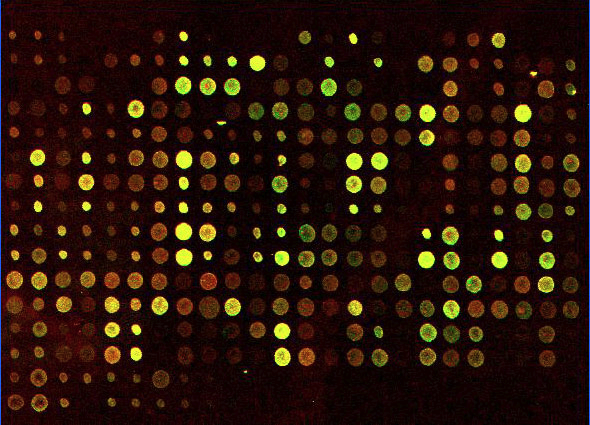
\includegraphics[width=10cm]{images/expresso-screenshot.png}
  \caption{Пример изображения микропробы в Expresso. Микропроба выводится в четырех квадрантах 24x16, один из которых представлен на этом рисунке.}
  \label{fig:expresso-screenshot}
\end{figure}

Проект Expresso направлен на поддержку всего цикла исследований в микропробной биоинформатике, области, в которой ``вычислительные системы в связке со сложными инженерными инструментами облегчают исследования в специализированных областях, таких как генетика, окружающая среда и создание лекарств''.
                                                                                                        
Expresso PSE разработана для поддержки всех работ, связанных с методом microarray, включая разработку эксперимента, сбор данных, обработка изображений, статистический анализ и data-mining. Архитектура Expresso включает в себя модели биофизических и биохимических процессов (для поддержки моделирования экспериментов). Далее в работу вступает сложные модули, использующие алгоритмы робототехники, физической химии и молекулярной биологии. Как только модель эксперимента подготовлена, Expresso постоянно адаптирует различные стадии эксперимента, отслеживая их прогресс и используя уже полученную информацию для выдачи рекомендаций по дальшейшим стадиям экперимента. На данном этапе, прототимы последних трех стадий эксперимента (обработка изображений, статистический анализ и data mining) полностью автоматизированы и интегрированы в реализацию системы.

Дизайн Expresso подчеркивает важность моделирования физических и вычислительных процессов, связанных друг с другом, что помогает улучшить биологическую модель и генерацию гипотез. Таким образом, возможность предоставления простого и высокопроизводительного доступа к объектам и потокам (для управления экспериментом) с минимальными затратами (в терминах традиционной функциональности баз данных, такой как управление транзакциями и поддержка целостности), является уникальной особенностью Expresso.

Процессы моделирования, анализа и data-mining-а в методе микропроб являются строго интерактивными и итеративными. Expresso использует легковесную модель данных как для разарботки экспериментов, так и для анализа данных. Система ведет базу данных решенных проблем и использует data mining чтобы улучшить будущие эксперименты основываясь на результатах уже проведенных, похожих опытов. Expresso также использует индуктивное логическое программирование, одну из техник data-mining, чтобы моделировать взаимодействия между генами и вычислять предполагаемые генные регуляторные механизмы. Одной из многочисленных стадий проекта Expresso было изучение генных шаблонов сосен, выполненное в ходе совместного проекта с группой изучения биотехнологий леса Государственного университета Северной Каролины.
  
\textbf{Выводы:} распределенная вычислительная среда при помощи специальных аппаратных средств может использоваться, в том числе, и для контроля за ходом реальных экспериментов. Также, применение алгоритмов data-mining к результатам уже проведенных опытов может существенно помочь при решении различных задач.
